\chapter{Standard Template Library}

The Standard Template Library (STL) is a collection of C++ template classes that provide general-purpose data structures and algorithms, including \texttt{std::vector}, \texttt{std::list}, \texttt{std::queue}, and \texttt{std::stack}. The STL consists of four main components:

\begin{itemize}
    \item \textbf{Algorithms}: A collection of functions designed to operate on ranges of elements.
    \item \textbf{Containers}: Objects that store collections of other objects.
    \item \textbf{Function Objects}: Components that allow the creation of callable objects.
    \item \textbf{Iterators}: Objects that enable traversal of a container.
\end{itemize}

\section{Containers}

Containers are objects that store data. The STL provides several container classes, each supporting different operations. STL containers are categorized as follows:

\begin{itemize}
    \item \textbf{Sequence Containers}: These containers maintain ordered collections of elements. The main sequence containers are \texttt{std::vector}, \texttt{std::list}, and \texttt{std::deque}.
    \item \textbf{Associative Containers}: These containers store elements in sorted order and support fast searching. The main associative containers are \texttt{std::set}, \texttt{std::multiset}, \texttt{std::map}, and \texttt{std::multimap}.
    \item \textbf{Container Adaptors}: These provide restricted access to elements by adapting existing containers. The primary container adaptors are 	exttt{std::stack}, 	exttt{std::queue}, and 	exttt{std::priority\_queue}.
    \item \textbf{Special Containers}: These containers provide specialized functionality. Examples include \texttt{std::byte}, \texttt{std::pair}, \texttt{std::tuple}, \texttt{std::variant}, \texttt{std::optional} and \texttt{std::any}.
\end{itemize}

\subsection{Sequence Containers}

Sequence containers maintain ordered collections of elements, with element positions independent of their values. In \texttt{std::vector} and \texttt{std::array}, elements are stored contiguously in memory and can be accessed using an index \texttt{[]}.

Examples of sequence containers include \texttt{std::vector<T>}, \texttt{std::array<T,N>}, \texttt{std::deque<T>}, and \texttt{std::list<T>}.

\begin{exampleblock}
    \begin{codeblock}[language=C++]
#include <iostream>
#include <vector>

int main() {
    std::vector<int> v = {1, 2, 3, 4, 5};
    for (int num : v) {
        std::cout << num << " ";
    }
    return 0;
}
    \end{codeblock}
\end{exampleblock}

\subsection{Associative Containers}

Associative containers store elements in sorted order and support fast searching. The main associative containers are \texttt{std::set}, \texttt{std::multiset}, \texttt{std::map}, and \texttt{std::multimap}.

\begin{itemize}
    \item \texttt{std::set} is a container that stores unique elements in sorted order. Here, \textbf{key} and \textbf{value} are the same and thus used interchangeably.
    \item \texttt{std::multiset} is a container that stores multiple elements in sorted order.
    \item \texttt{std::map} is a container that stores key-value pairs in sorted order.
    \item \texttt{std::multimap} is a container that stores multiple key-value pairs in sorted order.
\end{itemize}

\begin{exampleblock}
    \begin{codeblock}[language=C++]
#include <iostream>

int main() {
    std::map<std::string, int> m;
    m["one"] = 1;
    m["two"] = 2;
    m["three"] = 3;

    for (const auto& [key, value] : m) {
        std::cout << key << " => " << value << std::endl;
    }
    return 0;
}
    \end{codeblock}
\end{exampleblock}

They can be further divided in \textbf{ordered} and \textbf{unordered} associative containers. The former maintain elements in sorted order, while the latter do not.
For the former, an ordering relation is required for the elements, which can be provided by a comparison function or by a comparison operator. Moreover, keys can be accessed read-only, but not modified.
For the latter, a hashing function is required for the elements, which can be provided by a hash function or by a hash operator. Keys can be accessed and modified.

\subsection{Container Adaptors}

Container adaptors provide restricted access to elements by adapting existing containers. The primary container adaptors are \texttt{std::stack}, \texttt{std::queue}, and \texttt{std::priority\_queue}.
\begin{itemize}
    \item \texttt{std::stack} is a container that provides a LIFO (Last In, First Out) data structure.
    \item \texttt{std::queue} is a container that provides a FIFO (First In, First Out) data structure.
    \item \texttt{std::priority\_queue} is a container that provides a priority queue data structure.
\end{itemize}

\begin{exampleblock}
    \begin{codeblock}[language=C++]
#include <iostream>
#include <queue>

int main() {
    std::queue<int> q;
    q.push(1);
    q.push(2);
    q.push(3);

    while (!q.empty()) {
        std::cout << q.front() << " ";
        q.pop();
    }
    return 0;
}

    \end{codeblock}
\end{exampleblock}

\subsection{Special Containers}

Special containers provide specialized functionality. Examples include \texttt{std::byte}, \texttt{std::pair}, \texttt{std::tuple}, \texttt{std::variant}, \texttt{std::optional}, and \texttt{std::any}.
\begin{itemize}
    \item \texttt{std::byte} is a container that stores byte values.
    \item \texttt{std::pair} is a container that stores a pair of elements.
    \item \texttt{std::tuple} is a container that stores a tuple of elements.
    \item \texttt{std::variant} is a container that stores a variant of elements.
    \item \texttt{std::optional} is a container that stores an optional value.
    \item \texttt{std::any} is a container that stores any type of value.
\end{itemize}

\begin{exampleblock}
    \begin{codeblock}[language=C++]
#include <iostream>
#include <tuple>

int main() {
    std::tuple<int, float, std::string> t(1
    , 3.14, "Hello");
    std::cout << std::get<0>(t) << " ";
    std::cout << std::get<1>(t) << " ";

    return 0;
}
    \end{codeblock}
\end{exampleblock}

For further examples see \href{https://en.cppreference.com/w/cpp/container}{here}.


\subsection{Iterators}

Iterators are a generalization of \textbf{pointers} that allow a C++ program to work with different data
structures (for example, containers and ranges (since C++20)) in a uniform manner. The iterator
library provides definitions for iterators, as well as iterator traits, adaptors, and utility functions.

\begin{definitionblock}
    An iterator is any object that allows iterating over a succession of elements, typically stored in a
    standard container. It can be dereferenced with the \plaintt{*} operator, returning an element of the
    range, and incremented (moving to the next element) with the \plaintt{++} operator.
\end{definitionblock}

\begin{figure}[H]
    \centering
    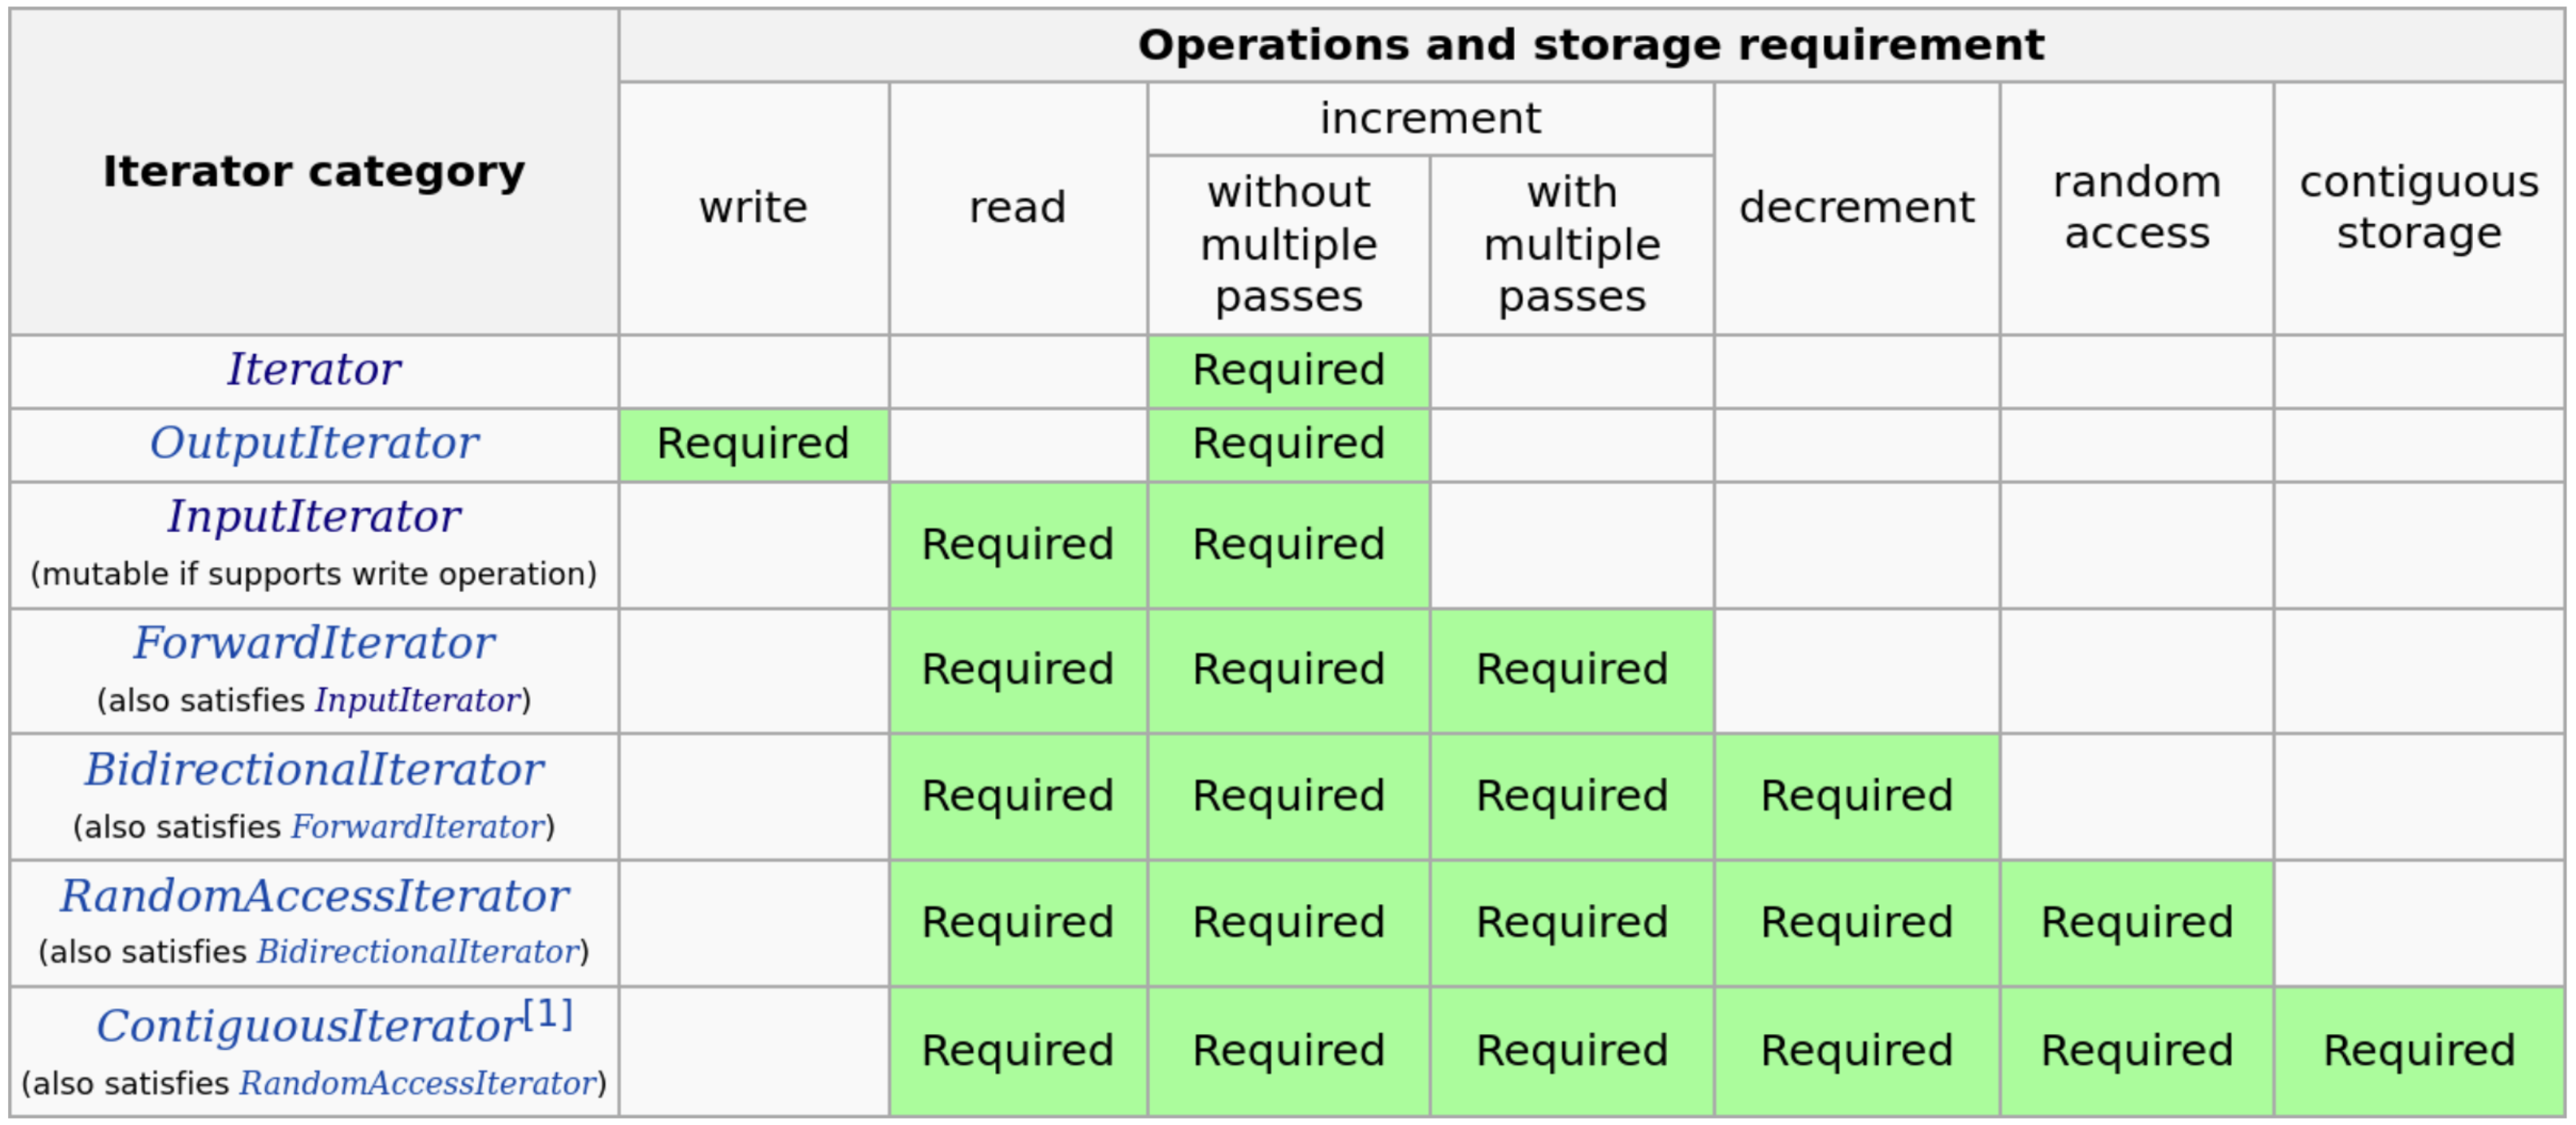
\includegraphics[width=\textwidth]{assets/iterators.png}
    \caption{Iterators}
\end{figure}

\subsection*{Key Concepts of Iterators}
\begin{itemize}
    \item \textbf{Abstraction}: Iterators provide a way to access elements of a container without exposing its internal structure.
    \item \textbf{Uniform Interface}: They offer a consistent interface for traversing different types of containers (e.g., arrays, vectors, lists, etc.).
    \item \textbf{Categories}: Iterators are categorized based on their functionality. The main categories are:
    \begin{itemize}
        \item \textbf{Input Iterators}: Can read elements in a sequence (forward-only, single-pass).
        \item \textbf{Output Iterators}: Can write elements in a sequence (forward-only, single-pass).
        \item \textbf{Forward Iterators}: Can read and write elements in a sequence (forward-only, multi-pass).
        \item \textbf{Bidirectional Iterators}: Can move both forward and backward in a sequence.
        \item \textbf{Random Access Iterators}: Can access any element in constant time (like pointers).
    \end{itemize}
\end{itemize}

\subsection*{Common Iterator Operations}
\begin{itemize}
    \item \texttt{*iter}: Dereference the iterator to access the element it points to.
    \item \texttt{iter->member}: Access a member of the element the iterator points to.
    \item \texttt{++iter} / \texttt{iter++}: Move the iterator to the next element.
    \item \texttt{--iter} / \texttt{iter--}: Move the iterator to the previous element (for bidirectional and random access iterators).
    \item \texttt{iter1 == iter2} / \texttt{iter1 != iter2}: Compare two iterators for equality.
    \item \texttt{iter + n} / \texttt{iter - n}: Move the iterator by \texttt{n} positions (for random access iterators).
\end{itemize}

\subsection*{Iterator Types in C++ Standard Library}
\begin{itemize}
    \item \texttt{begin()} and \texttt{end()}:
    \begin{itemize}
        \item \texttt{begin()} returns an iterator to the first element of the container.
        \item \texttt{end()} returns an iterator to one past the last element (used as a sentinel value).
    \end{itemize}
    \item \texttt{const\_iterator}: A read-only iterator that cannot modify the elements of the container.
    \item \texttt{reverse\_iterator}: Iterates over the container in reverse order.
\end{itemize}
\begin{exampleblock}
\begin{codeblock}[language=C++]
#include <iostream>
#include <vector>

int main() {
    std::vector<int> vec = {1, 2, 3, 4, 5};

    // Using iterators to traverse the vector
    for (auto it = vec.begin(); it != vec.end(); ++it) {
        std::cout << *it << " "; // Dereference the iterator to access the element
    }
    std::cout << std::endl;

    // Using range-based for loop (internally uses iterators)
    for (int val : vec) {
        std::cout << val << " ";
    }
    std::cout << std::endl;

    return 0;
}
\end{codeblock}
\end{exampleblock}

\subsection*{Iterator Categories in Practice}
\begin{itemize}
    \item \textbf{Random Access Iterators}: Supported by \texttt{std::vector}, \texttt{std::array}, and \texttt{std::deque}.
    \item \textbf{Bidirectional Iterators}: Supported by \texttt{std::list} and \texttt{std::set}.
    \item \textbf{Forward Iterators}: Supported by \texttt{std::forward\_list}.
    \item \textbf{Input/Output Iterators}: Used in specific scenarios like reading from or writing to streams.
\end{itemize}

\subsection*{Custom Iterators}
You can also define custom iterators for your own container classes by implementing the required operations (e.g., \texttt{++}, \texttt{*}, \texttt{==}, etc.).

\subsection{size\_type and size\_t}

They are used to represent the size of a container. \texttt{size\_type} is a type defined by the container class, while \texttt{size\_t} is a type defined by the C++ standard library.
They are guaranteed to be unsigned integral types, but their sizes may vary depending on the platform.

\begin{exampleblock}
\begin{codeblock}[language=C++]
#include <iostream>
#include <vector>

int main() {
    std::vector<int> vec = {1, 2, 3, 4, 5};
    std::vector<int>::size_type vec_size = vec.size();
    std::size_t vec_size_t = vec.size();

    std::cout << "size_type: " << vec_size << std::endl;
    std::cout << "size_t: " << vec_size_t << std::endl;

    return 0;
}
\end{codeblock}
\end{exampleblock}

\section{Algorithms}

The STL provides an extensive set of algorithms to operate on containers, or more precisely on
\textbf{ranges}.

\begin{warningblock}
    C++20 has revised the concept of range and provides a new set of algorithms in the
    namespace \plaintt{std::ranges} , with the same name as the old ones, but simpler to use
    and sometimes more powerful.
\end{warningblock}

\subsection*{Why use STL Algorithms?}

With standardized algorithms:
\begin{itemize}
    \item You are more uniform with respect to different container types.
    \item The algorithm of the standard library may do certain optimizations if the contained elements have some characteristics.
    \item You have a parallel version for free$\dots$
\end{itemize}

\subsection{Non-modifying Algorithms}

Non-modifying algorithms do not change the contents of the container (the value in the range). They are used to perform operations like searching, counting, and comparing elements.

\begin{exampleblock}
\begin{codeblock}[language=C++]
#include <iostream>
#include <vector>
#include <algorithm>

int main() {
    std::vector<int> vec = {1, 2, 3, 4, 5};

    // Find the first element greater than 3
    auto it = std::find_if(vec.begin(), vec.end(), [](int x) { return x > 3; });

    if (it != vec.end()) {
        std::cout << "First element greater than 3: " << *it << std::endl;
    }

    // Check if all elements are positive
    bool all_positive = std::all_of(vec.begin(), vec.end(), [](int x) { return x > 0; });

    if (all_positive) {
        std::cout << "All elements are positive" << std::endl;
    }

    return 0;
}
\end{codeblock}
\end{exampleblock}

\subsection{Modifying Algorithms}

Modifying algorithms change the contents of the container. They are used to perform operations like sorting, removing elements, and transforming elements.

\begin{exampleblock}
\begin{codeblock}[language=C++]
#include <iostream>
#include <vector>
#include <algorithm>

int main() {
    std::vector<int> vec = {5, 2, 3, 4, 1};

    // Sort the elements in ascending order
    std::sort(vec.begin(), vec.end());

    // Remove the first element
    vec.erase(vec.begin());

    // Transform each element to its square
    std::transform(vec.begin(), vec.end(), vec.begin(), [](int x) { return x * x; });

    for (int val : vec) {
        std::cout << val << " ";
    }
    std::cout << std::endl;

    return 0;
}
\end{codeblock}
\end{exampleblock}

\subsection{Inserters}

Inserters are used to insert elements into a container. The main inserters are:
\begin{itemize}
    \item \texttt{std::back\_inserter}: Inserts elements at the end of a container.
    \item \texttt{std::front\_inserter}: Inserts elements at the beginning of a container.
    \item \texttt{std::inserter}: Inserts elements at a specified position in a container.
\end{itemize}

\begin{exampleblock}
\begin{codeblock}[language=C++]
#include <iostream>
#include <vector>
#include <algorithm>

int main() {
    std::vector<int> vec1 = {1, 2, 3};
    std::vector<int> vec2 = {4, 5, 6};

    // Insert elements from vec2 to vec1
    std::copy(vec2.begin(), vec2.end(), std::back_inserter(vec1));

    for (int val : vec1) {
        std::cout << val << " ";
    }
    std::cout << std::endl;

    return 0;
}
\end{codeblock}
\end{exampleblock}

\subsection{Sorting Algorithms}

Sorting algorithms are used to arrange elements in a specific order. They operate on a range to order it according to an ordering relation. 

\begin{exampleblock}
\begin{codeblock}[language=C++]
#include <iostream>
#include <vector>
#include <algorithm>

int main() {
    std::vector<int> vec = {5, 2, 3, 4, 1};

    // Sort the elements in ascending order
    std::sort(vec.begin(), vec.end());

    for (int val : vec) {
        std::cout << val << " ";
    }
    std::cout << std::endl;

    return 0;
}
\end{codeblock}
\end{exampleblock}

\subsection{Min and Max}

They are used to find the minimum and maximum elements in a range. The functions \texttt{std::min\_element} and \texttt{std::max\_element} return an iterator to the minimum and maximum elements, respectively.

\begin{exampleblock}
\begin{codeblock}[language=C++]
#include <iostream>
#include <vector>
#include <algorithm>

int main() {
    std::vector<int> vec = {5, 2, 3, 4, 1};

    // Find the minimum and maximum elements
    auto min_it = std::min_element(vec.begin(), vec.end());
    auto max_it = std::max_element(vec.begin(), vec.end());

    std::cout << "Min element: " << *min_it << std::endl;
    std::cout << "Max element: " << *max_it << std::endl;

    return 0;
}
\end{codeblock}
\end{exampleblock}

\subsection{Numeric Algorithms}

Numeric algorithms are used to perform numeric operations on a range of elements. The main numeric algorithms are:

\begin{itemize}
    \item \texttt{std::accumulate}: Computes the sum of elements in a range.
    \item \texttt{std::inner\_product}: Computes the inner product of two ranges.
    \item \texttt{std::partial\_sum}: Computes the partial sum of elements in a range.
    \item \texttt{std::adjacent\_difference}: Computes the differences between adjacent elements in a range.
\end{itemize}

\begin{exampleblock}
\begin{codeblock}[language=C++]
#include <iostream>
#include <vector>
#include <numeric>

int main() {
    std::vector<int> vec = {1, 2, 3, 4, 5};

    // Compute the sum of elements
    int sum = std::accumulate(vec.begin(), vec.end(), 0);

    // Compute the partial sum of elements
    std::vector<int> partial_sum(vec.size());
    std::partial_sum(vec.begin(), vec.end(), partial_sum.begin());

    for (int val : partial_sum) {
        std::cout << val << " ";
    }
    std::cout << std::endl;

    return 0;
}
\end{codeblock}
\end{exampleblock}




\section{STL evolution}

The STL has evolved over time, with new features and improvements introduced in each C++ standard. Here are some key changes in the STL from C++11 to C++20:

\begin{itemize}
    \item \textbf{C++11}: Introduced move semantics, lambda expressions, and range-based for loops.
    \item \textbf{C++14}: Added generic lambdas, variable templates, and binary literals.
    \item \textbf{C++17}: Introduced parallel algorithms, \texttt{std::optional}, \texttt{std::variant}, and \texttt{std::any}.
    \item \textbf{C++20}: Added concepts, ranges, coroutines, and \texttt{std::span}.
\end{itemize}

\subsection*{For loop evolution}

The range-based for loop was introduced in C++11 to simplify iteration over containers. It allows you to iterate over a range of elements without using iterators explicitly.

\begin{exampleblock}
\begin{codeblock}[language=C++]
#include <iostream>
#include <vector>

int main() {
    std::vector<int> vec = {1, 2, 3, 4, 5};

    // Using range-based for loop
    for (int val : vec) {
        std::cout << val << " ";
    }
    std::cout << std::endl;

    return 0;
}
\end{codeblock}
\end{exampleblock}






\newpage
\section{Smart Pointers}

\begin{definitionblock}[RAII]
    \textbf{Resource Acquisition Is Initialization} plays a significant role in C++. It essentially means that an object should be responsible for both the creation and destruction of the resources it owns.
\end{definitionblock}

\begin{exampleblock}[RAII Compliant]
    \begin{codeblock}[language=C++]
std::array<double, 10> p;  // var p creates and destroys the array
    \end{codeblock}
\end{exampleblock}

In C++, \textbf{smart pointers} are important tools to implement RAII.

Types of pointers:
\begin{itemize}
    \item \textbf{Standard Pointers}: use them only to watch and operate on an object whose lfespan is independent of the one of the pointer.
    \item \textbf{Smart Pointers}: they control the lifespan of an object. 
    \begin{itemize}
        \item \texttt{std::unique\_ptr}: manages a single object. The owned resource is destroyed when the pointer goes out of scope.
        \item \texttt{std::shared\_ptr}: manages a shared object. The owned resource is destroyed when the \textbf{last} shared pointer goes out of scope.
        \item \texttt{std::weak\_ptr}: observes a shared object without owning it. It is used to break circular references between \texttt{std::shared\_ptr}s.
    \end{itemize}
\end{itemize}

\begin{exampleblock}
    \begin{codeblock}[language=C++] 
#include <iostream>

class MyClass {
public:
        set_polygon(std::unique_ptr<Polygon> p) {
            polygon = std::move(p);
        }
private:
        std::unique_ptr<Polygon> polygon;
};

std::unique_ptr<Polygon> create_polygon() {
    switch(t){
        case "Triangle":
            return std::make_unique<Triangle>();
        case "Rectangle":
            return std::make_unique<Rectangle>();
        default:
            return nullptr;
    }
}

MyClass obj;
obj.set_polygon(create_polygon("Triangle"));

    \end{codeblock}
\end{exampleblock}

\subsection{std::unique\_ptr}
A \texttt{std::unique\_ptr} serves as the unique owner of the object of type \texttt{T} it refers to. The object is destroyed automatically when the \texttt{std::unique\_ptr} goes out of scope.
It implements the \texttt{*} and \texttt{->} operators to access the object it owns, so it can be used as standard pointer, but can only be initialized through the constructor. 

The default contructor produces a \textbf{null pointer}. 

\begin{warningblock}[Copying]
    By definition, unique pointers cannot be \textbf{copied}, but their ownership can be transferred using the \plaintt{std::move} function. The previous owner will be left with a null pointer.
\end{warningblock}

\subsection{std::shared\_ptr}

For instance you have several objects that refer to a resource (e.g., a matrix, a shape, ...) that is
build dynamically (and maybe is a polymorphic object). You want to keep track of all the
references in such a way that when (and only when) the last one gets destroyed the resource is
also destroyed.

A \texttt{Shared Pointer} implements the semantics of \textit{clean it up} when the resource is no longer needed. 

\begin{exampleblock}
    \begin{codeblock}[language=C++]
#include <iostream>

class MyClass { ... };

class Preprocessor {
public: 
    Preprocessor(std::shared_ptr<Data> &data, ...) : data(data) {}
private:
    std::shared_ptr<Data> data;
};

class NumericalSolver {
public:
    NumericalSolver(std::shared_ptr<Data> &data, ...) : data(data) {}
private:
    std::shared_ptr<Data> data;
};

int main() {
    std::shared_ptr<Data> data = std::make_shared<Data>();
    Preprocessor preprocessor(data, ...);
    preprocessor.preprocess();
    // shared\_data will still be used by other resources, hence it cannot be destroyed here.
    NumericalSolver solver(data, ...);
    solver.solve();
    return 0;
}
    \end{codeblock}
\end{exampleblock}

\subsubsection*{How a shared pointer works}
The \texttt{std::shared\_ptr} keeps track of the number of shared references to an object through reference counting. 
When the reference count
reaches zero, the object is automatically deallocated, preventing memory leaks.
It implements \texttt{*} and \texttt{->} operators to access the object it owns, so it can be used as a standard pointer.
Moreover, it provides copy constructors and assignment operators.


\subsection{std::weak\_ptr}
The \texttt{std::weak\_ptr} is a smart pointer that holds a non-owning (weak) reference to an object
managed by a \texttt{std::shared\_ptr}. It is used to break circular references between shared pointers.
It must also be converted to a \texttt{std::shared\_ptr} to access the object it refers to.

\begin{exampleblock}
    \begin{codeblock}[language=C++]
#include <iostream>

std::shared_ptr<int> shared = std::make_shared<int>(42);
std::weak_ptr<int> weak = shared;  // Get pointer to data without taking ownership.
    \end{codeblock}
\end{exampleblock}



\section{Move Semantics}

\textbf{Problem}: how can I swap two objects in an efficient way?

Before C++11 one could have used a special method or a friend function. 

\begin{exampleblock}
    \begin{codeblock}[language=C++]
#include <iostream>

void swap_with_move(Matrix& a, Matrix& b) {
    // swap rows and cols 

    double* tmp = a.data; // save the pointer 
    a.data = b.data // copy the pointer
    b.data = tmp; // copy the pointer
}
    \end{codeblock}
\end{exampleblock}

But this way it is not generalizable, since I cannot write a function template \texttt{swap\_with\_move<T>}, because I need to know how data is stored in \texttt{T} for each case.

\subsection*{Lvalues}
\begin{definitionblock}
    An \textbf{lvalue} (left value) is an expression that refers to a specific memory location and persists beyond a single expression.
\end{definitionblock}

\begin{itemize}
    \item They have an \textbf{identifiable memory location}.
    \item They can be \textbf{modified} (unless they are \texttt{const}).
    \item They can be \textbf{bound to lvalue references} (\texttt{T\&}).
\end{itemize}

\begin{exampleblock}
\begin{codeblock}[language=C++]
int x = 10;  // 'x' is an lvalue
x = 20;      // Valid: lvalues can appear on the left side of an assignment

int& ref = x;  // Valid: lvalues can be bound to lvalue references
\end{codeblock}
\end{exampleblock}

A \texttt{const} lvalue is still an lvalue but cannot be modified:
\begin{codeblock}[language=C++]
const int y = 5;
y = 10;  // Error: lvalue is read-only
\end{codeblock}

\subsection*{Rvalues}
\begin{definitionblock}
    An \textbf{rvalue} (right value) is an expression that does \textbf{not persist beyond a single expression} and does not have a specific memory location that can be accessed.
\end{definitionblock}

\begin{itemize}
    \item They are \textbf{temporary} and cannot be assigned to.
    \item They \textbf{cannot be bound to lvalue references} (\texttt{T\&}), but they \textbf{can be bound to rvalue references} (\texttt{T\&\&}).
\end{itemize}

\begin{exampleblock}
\begin{codeblock}[language=C++]
int x = 10;
int y = x + 5;  // 'x + 5' is an rvalue
\end{codeblock}
\end{exampleblock}

C++11 introduced \textbf{rvalue references} to allow functions to take ownership of temporary values:
\begin{codeblock}[language=C++]
void foo(int&& a) {  // Accepts only rvalues
    std::cout << "Rvalue: " << a << std::endl;
}

foo(10);  // Valid: '10' is an rvalue
int x = 5;
foo(x);   // Error: 'x' is an lvalue
\end{codeblock}

\subsection*{Lvalues vs. Rvalues in Function Overloading}
Functions can be overloaded based on lvalue and rvalue references:
\begin{codeblock}[language=C++]
void process(int& x) {
    std::cout << "Lvalue reference" << std::endl;
}

void process(int&& x) {
    std::cout << "Rvalue reference" << std::endl;
}

int main() {
    int a = 10;
    process(a);   // Calls lvalue version
    process(20);  // Calls rvalue version
}
\end{codeblock}


\subsection{How Move Semantics is implemented}

The following is the standard signature of a move operation for a class \texttt{Matrix}:
\begin{codeblock}[language=C++]
    Matrix(Matrix&&); // move constructor
    Matrix& operator=(Matrix&&); // move assignment operator
\end{codeblock}

\begin{exampleblock}
    \begin{codeblock}[language=C++]
#include <iostream>

Matrix(Matrix&& rhs) : data(rhs.data), nr(rhs.nr), nc(rhs.nc) {
    rhs.data = nullptr;
    rhs.nr = 0;
    rhs.nc = 0;
}

Matrix& operator=(Matrix&& rhs) {
    delete[] this -> data; // release the resource
    data = rhs.data; // shallow copy 
    // Fix rhs so it is a valid empty matrix
    rhs.data = nullptr;
    rhs.nr = 0;
    rhs.nc = 0;
}

int main() {
    Matrix foo();
    // ... 
    Matrix a;
    a = foo(); // move assignment is called 
    return 0;
}
    \end{codeblock}
\end{exampleblock}

\begin{observationblock}[std::move]
    The \texttt{std::move} function is used to convert an lvalue to an rvalue reference, allowing it to be moved instead of copied. It basically cast the value to an rvalue, making it available to be copied. 
\end{observationblock}

\begin{codeblock}[language=C++]
    template<class T>
    void swap(T& a, T& b) {
        T tmp = std::move(a);
        a = std::move(b);
        b = std::move(tmp);
    }
    // or simpler 
    std::swap(a, b);
\end{codeblock}

The solution is to force the move:
\begin{codeblock}[language=C++]
    class Foo{
    public:
        Foo(Matrix&& m) : my_m(std::move(m)) {}
        // ... 
    private:
        Matrix my_m;
    }
\end{codeblock}

Now, m is moved into my\_m. 

\textbf{All} standard containers support move semantic, and all standard algorithms are written so
that if the contained type implements move semantics, the creation of unnecessary temporaries
can be avoided. All containers also have a \texttt{swap()} method that performs swaps intelligently.





\section{Exceptions}

A \textbf{function} can be seen as a mapping from input data to output data. 
The conditions under which the input data is considered valid is called \textbf{precondition}, 
while the conditions under which the output data is considered valid is called \textbf{postcondition}.
Failure to meet these conditions is considered a \textbf{failure} or \textbf{bug}.

An \textbf{invariant} is a condition that must always be true during the execution of a program.
    An object is considered to be in an \textbf{inconsistent state} if the invariants are not met.

\begin{definitionblock}[Exception]
    An \textbf{exception} is an anomalous condition that disrupts the normal flow of a program's execution
    when left unhandled. It is not the result of incorrect coding but rather arises from challenging or
    unpredictable circumstances.
\end{definitionblock}


\subsection{Run-time assertions}

\begin{exampleblock}
    \begin{codeblock}[language=C++]
double calculate(double operand1, double operand2) {
    assert(operand2 != 0.0 && "Division by zero");
    return operand1 / operand2;
}
    \end{codeblock}
\end{exampleblock}

For improved efficiency, all assertions can be disabled by defining the \texttt{NDEBUG} macro:
\begin{codeblock}[language=bash]
    g++ -DNDEBUG -o program program.cpp
\end{codeblock}


\subsection{Compile-time assertions}

\begin{exampleblock}
    \begin{codeblock}[language=C++]
template <typename T>
void process(T value) {
    static_assert(std::is_integral<T>::value, "T must be an integral type");
    // Process the value
}
    \end{codeblock}
\end{exampleblock}
If the condition is met, the error message is printed to the standard error and compilation will fail.


\subsection{Exception handling in C++}

The basic structure to handle exceptions is:
\begin{itemize}
    \item Using the \texttt{throw} command to indicate that an exception has occurred. You can throw an
    object containing information about the exception.
    \item Employing the \texttt{try-catch} blocks to catch and handle exceptions. If an exception is not
    caught, it will propagate up the call stack and might lead to program termination.
\end{itemize}

\begin{exampleblock}
    \begin{codeblock}[language=C++]
int divide(int dividend, int divisor) {
    if (divisor == 0) {
        throw std::runtime_error("Division by zero");
    }
    return dividend / divisor;
}

try{
    const int result = divide(10, 0);
    std::cout << "Result: " << result << std::endl;
} catch (const std::runtime_error& e) {
    std::cerr << "Exception: " << e.what() << std::endl;
}
    \end{codeblock}
\end{exampleblock}

Standard exceptions examples are:
\begin{itemize}
    \item \texttt{std::exception}: Base class for all standard exceptions.
    \item \texttt{std::runtime\_error}: Exception used to report runtime errors.
    \item \texttt{std::logic\_error}: Exception used to report errors in the program's logic.
    \item \texttt{std::invalid\_argument}: Exception used to report invalid arguments.
    \item \texttt{std::out\_of\_range}: Exception used to report out-of-range errors.
    \item \texttt{std::bad\_alloc}: Exception used to report memory allocation errors.
    \item \texttt{std::bad\_cast}: Exception used to report casting errors.
\end{itemize}

\begin{observationblock}
    In situations where an algorithm's failure is one of its expected outcomes (e.g., the failure of
    convergence in an iterative method), returning a \textbf{status} rather than throwing an exception may be
    more suitable. Instead of terminating the program, a status variable is used to indicate the
    outcome, which can be checked by the caller. See also \plaintt{std::terminate} , \plaintt{std::abort} and \plaintt{std::exit}.
\end{observationblock}

Note, also, that \textbf{floating-point exceptions} do not result in program failure, instead they produce special numerical values like \texttt{NaN} or \texttt{Inf}, and the operations continue. 


\section{STL Utilities}

\subsection{I/O Streams}

Input/Output (I/O) streams in C++ provide a convenient way to perform input and output
operations, allowing you to work with various data sources and destinations, such as files,
standard input/output, strings, and more.

The key components are:
\begin{itemize}
    \item \textbf{iostream}: Provides the basic input/output operations. It is used for interacting with the standard input and output streams.
    \item \textbf{ifstream}: This class is used for reading data from files. You can open a file for input and
    read data from it.
    \begin{codeblock}[language=C++]
        std::ifstream file("input.txt");

        if (file.is_open()) {
            std::string line;
            while (std::getline(file, line)) {
                std::cout << line << std::endl;
            }
            file.close();
        } else {
            std::cerr << "Failed to open the file." << std::endl;
        }
    \end{codeblock}
    \item \textbf{ofstream}: This class is used for writing data to files. You can open a file for output and write data to it.
    \begin{codeblock}[language=C++]
        std::ofstream file("output.txt");

        if (file.is_open()) {
            file << "Hello, World!" << std::endl;
            file.close();
        } else {
            std::cerr << "Failed to open the file." << std::endl;
        }
    \end{codeblock}
    \item \textbf{stringstream}: This class is used for reading and writing data to and from strings. It provides a way to work with strings as if they were streams.
    \begin{codeblock}[language=C++]
        std::stringstream ss;
        ss << "Hello, World!";
        std::string str = ss.str();
        std::cout << str << std::endl;

        // Passing data from a string using std::stringstream.
        std::string data = "42 3.14 Hello";
        std::stringstream ss(data);
        int num;
        double d;
        std::string word;
        ss >> num >> d >> word;
    \end{codeblock}
\end{itemize}

\subsection{Random Numbers}

The capability of generating random numbers is essential not only for statistical purposes but also
for internet communications. But an algorithm is deterministic. However, several techniques have
been developed to generate pseudo-random numbers. They are not really random, but they show
a low level of auto-correlation.

To generate them, you need the \texttt{<random>} header, and the chosen design is bsed on two types of objects:
\begin{itemize}
    \item \textbf{Engines}: They are the source of randomness. They are used to generate random numbers.
    \item \textbf{Distributions}: They are used to transform the random numbers generated by the engine into a specific range.
\end{itemize}

\subsubsection*{Engines}
Random number engines generate pseudo-random numbers using seed data as an entropy
source. Several different classes of pseudo-random number generation algorithms are
implemented as templates that can be customized. 

For simplicity, the library provides predefined engines, such as \texttt{std::default\_random\_engine},
which balances efficiency and quality. There are also non-deterministic engines, like \texttt{std::random\_device}, which generate non-deterministic random numbers based on hardware
data.

\begin{exampleblock}
    \begin{codeblock}[language=C++]
std::default_random_engine engine;  // with default seed
std::default_random_engine engine(42);  // with seed 42
    \end{codeblock}
\end{exampleblock}

\subsubsection*{Distributions}

Distributions are template classes that implement a call operator () to transform a random
sequence into a specific distribution. You need to pass a random engine to the distribution to
generate numbers according to the desired distribution. For example:

\begin{exampleblock}
    \begin{codeblock}[language=C++]
std::random_device rd;
std::default_random_engine engine(rd());
std::uniform_int_distribution<int> dist(1, 6);  // [1, 6]
int num = dist(engine);
    \end{codeblock}
\end{exampleblock}

\subsection{Shuffling}

In C++ you can shuffle a range of elements using the \texttt{std::shuffle} algorithm from the \texttt{<algorithm>} header. It rearranges the elements in the range \texttt{[first, last)} randomly using a random number generator.

\begin{exampleblock}
    \begin{codeblock}[language=C++]
std::vector<int> vec = {1, 2, 3, 4, 5};
std::random_device rd;
std::mt19937 engine(rd());
std::shuffle(vec.begin(), vec.end(), engine);
    \end{codeblock}
\end{exampleblock}

\subsection{Sampling}

The \texttt{std::sample} algorithm from the \texttt{<algorithm>} header is used to sample elements from a range. It selects a random subset of elements from the input range and stores them in the output range.

\begin{exampleblock}
    \begin{codeblock}[language=C++]
std::vector<int> vec = {1, 2, 3, 4, 5};
std::vector<int> sample(3);
std::random_device rd;
std::mt19937 engine(rd());
std::sample(vec.begin(), vec.end(), sample.begin(), 3, engine);
    \end{codeblock}
\end{exampleblock}

\subsection{Time Measuring}

C++ provides three types of clock:
\begin{itemize}
    \item \texttt{std::chrono::system\_clock}: Represents the system-wide real time wall clock.
    \item \texttt{std::chrono::steady\_clock}: Represents the monotonic clock that is not affected by system clock adjustments.
    \item \texttt{std::chrono::high\_resolution\_clock}: Represents the clock with the shortest tick period available on the system.
\end{itemize}

\begin{exampleblock}
    \begin{codeblock}[language=C++]
auto start = std::chrono::high_resolution_clock::now();
// Perform some operation
auto end = std::chrono::high_resolution_clock::now();
auto duration = std::chrono::duration_cast<std::chrono::milliseconds>(end - start);
    \end{codeblock}
\end{exampleblock}

\subsection{Filesystem Utilities}

The C++17 standard introduced the \texttt{<filesystem>} library, which provides facilities for performing operations on file systems and their components, such as paths, regular files, and directories.

\subsubsection*{Key Components}
\begin{itemize}
    \item \texttt{std::filesystem::path}: Represents a path in the filesystem.
    \item \texttt{std::filesystem::directory\_entry}: Represents a directory entry.
    \item \texttt{std::filesystem::directory\_iterator}: Iterates over the contents of a directory.
    \item \texttt{std::filesystem::recursive\_directory\_iterator}: Recursively iterates over the contents of a directory.
\end{itemize}

\subsubsection*{Common Operations}
\begin{itemize}
    \item \texttt{std::filesystem::exists}: Checks if a file or directory exists.
    \item \texttt{std::filesystem::create\_directory}: Creates a new directory.
    \item \texttt{std::filesystem::remove}: Removes a file or directory.
    \item \texttt{std::filesystem::rename}: Renames a file or directory.
    \item \texttt{std::filesystem::copy}: Copies a file or directory.
\end{itemize}

\begin{exampleblock}
\begin{codeblock}[language=C++]
#include <iostream>
#include <filesystem>

int main() {
    std::filesystem::path p = "example.txt";

    // Check if the file exists
    if (std::filesystem::exists(p)) {
        std::cout << p << " exists." << std::endl;
    } else {
        std::cout << p << " does not exist." << std::endl;
    }

    // Create a new directory
    std::filesystem::create_directory("new_directory");

    // Remove a file
    std::filesystem::remove("example.txt");

    // Rename a file
    std::filesystem::rename("old_name.txt", "new_name.txt");

    // Copy a file
    std::filesystem::copy("source.txt", "destination.txt");

    return 0;
}
\end{codeblock}
\end{exampleblock}

\subsubsection*{Iterating Over Directory Contents}
You can use \texttt{std::filesystem::directory\_iterator} to iterate over the contents of a directory.

\begin{exampleblock}
\begin{codeblock}[language=C++]
#include <iostream>
#include <filesystem>

int main() {
    std::filesystem::path dir = "some_directory";

    // Iterate over the contents of the directory
    for (const auto& entry : std::filesystem::directory_iterator(dir)) {
        std::cout << entry.path() << std::endl;
    }

    return 0;
}
\end{codeblock}
\end{exampleblock}

\subsubsection*{Recursive Directory Iteration}
You can use \texttt{std::filesystem::recursive\_directory\_iterator} to iterate over the contents of a directory recursively.

\begin{exampleblock}
\begin{codeblock}[language=C++]
#include <iostream>
#include <filesystem>

int main() {
    std::filesystem::path dir = "some_directory";

    // Recursively iterate over the contents of the directory
    for (const auto& entry : std::filesystem::recursive_directory_iterator(dir)) {
        std::cout << entry.path() << std::endl;
    }

    return 0;
}
\end{codeblock}
\end{exampleblock}


